\exercise{Spatial filtering}
\subsection*{a - Convolution}
Spatial filtering is an operation where each pixel is changed based on the values of the pixels in its neighborhood.
By performing these kinds of operations, interesting operations like blurring, sharpening or edge detection can be performed that are not possible with simple pointwise operations.

When performing spatial filtering on an image it is usually defined how a pixel is influenced by its neighborhood.
This definition is usually in the form of a matrix, which is called the mask or kernel.
By applying the mask to each pixel, a spatial filtered result is be obtained.
By iterating over the pixels in the image, and applying the mask to every pixel's neighborhood, one can retrieve an enhanced image.
This process is called convolution.

We have implemented this operation in the following \textit{MATLAB} code: 

\matlabexternal{IPfilter.m}

This function can convolute any image with a mask of any odd size.
To test that it behaves correctly we have applied a Gaussian kernel (as in Table~\ref{tbl:gauss}) to an image, which should result in a blurred version of the image.
Figures~\ref{fig:nonblur} and~\ref{fig:blur} illustrate the result.
\begin{figure}[!htb]
 \centering
 \begin{subfigure}[b]{0.49\linewidth}
  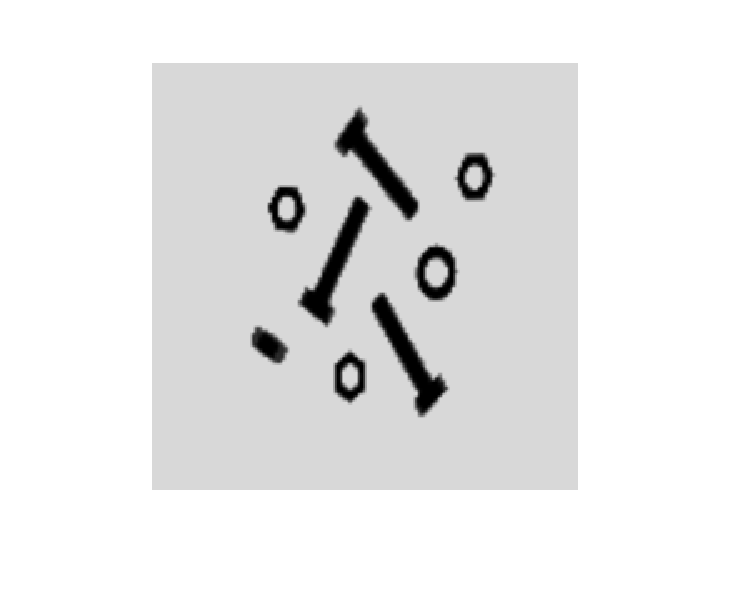
\includegraphics[width=\textwidth]{notBlurred.eps} 
  \caption{An image which was not blurred}
  \label{fig:nonblur} 
 \end{subfigure}
 \begin{subfigure}[b]{0.49\linewidth}
  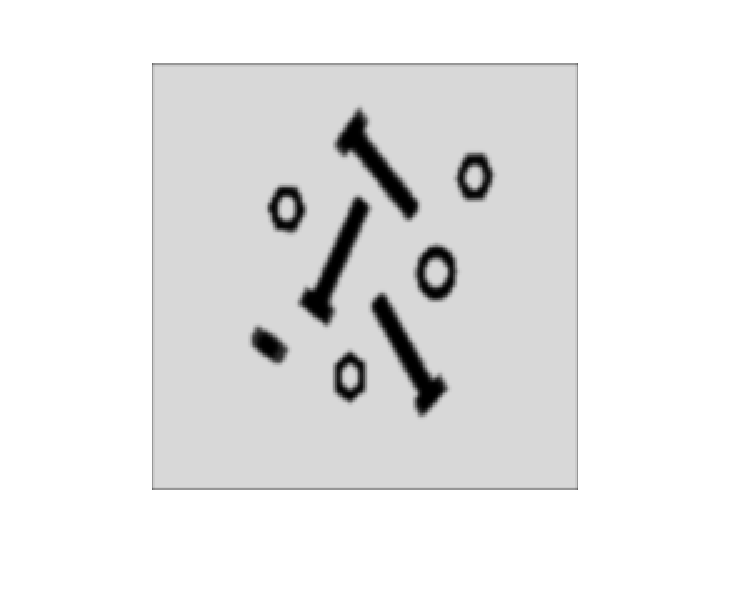
\includegraphics[width=\textwidth]{blurred.eps}
  \caption{The same image masked with a \(5\times5\) Gaussian kernel}
  \label{fig:blur}
 \end{subfigure}
 \caption{Gaussian mask applied to an image to demonstrate convolution}
\end{figure}
\begin{table}[!htb]
\begin{center}
$\frac{1}{273}$
\begin{tabular}{|c|c|c|c|c|}\hline
1 & 4 & 7 & 4 & 1\\ \hline
4 &  16 &  26 &  16 &  4 \\ \hline
7 &  26 &  41 &  26 &  7\\ \hline
4 &  16 &  26 &  16 &  4\\ \hline
1 &  4 &  7 &  4 &  1 \\ \hline
\end{tabular}

\caption{Gaussian kernel for blurring}
\label{tbl:gauss}
\end{center}
\end{table}

\subsection*{b - IPGradient}
We have also implemented the gradient magnitude computation. Normally this would mean that for each location $(x, y)$ of an image the rate of change in the direction of the gradient vector must be computed, which is $M(x, y) = mag(\nabla f) = \sqrt{g_x ^2 + g_y ^2}$. However, according to (3.6-18) of Digital Image Processing, this value is approximately equal to the Sobel operators. These matrices are defined as in table~\ref{tbl:sobel}. Using both these kernels and taking the sum of the absolute results of the convolutions of the original image, figures~\ref{fig:moonOrig} and~\ref{fig:moonSharp} are obtained. 
\begin{table}[!htb]
\begin{center}
\begin{tabular}{|c|c|c|}\hline
-1 & -2 & -1 \\ \hline
0 & 0 & 0 \\ \hline
1 & 2 & 1 \\ \hline
\end{tabular}
\begin{tabular}{|c|c|c|}\hline
-1 & 0 & 1 \\ \hline
-2 & 0 & 2 \\ \hline
-1 & 0 & 1 \\ \hline
\end{tabular}

\caption{Both the Sobel kernels for image sharpening}
\label{tbl:sobel}
\end{center}
\end{table}

\begin{figure}[!Hbt]
\centering
 \begin{subfigure}[b]{0.45\textwidth}
  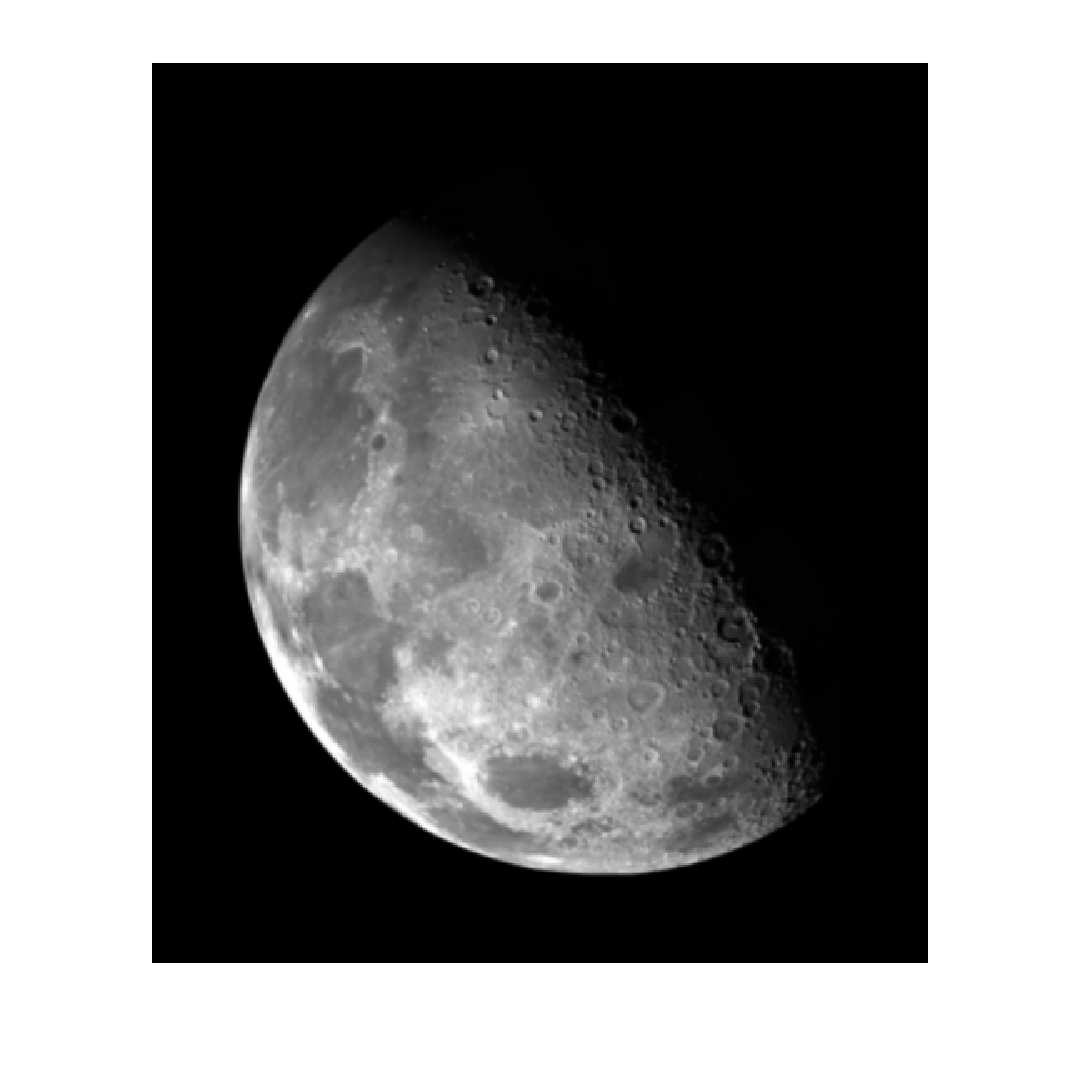
\includegraphics[width=\textwidth]{moonOriginal.eps}
  \caption{The original input images, a slightly blurred moon. \newline ~\newline}
  \label{fig:moonOrig}
 \end{subfigure}
 \begin{subfigure}[b]{0.45\textwidth}
  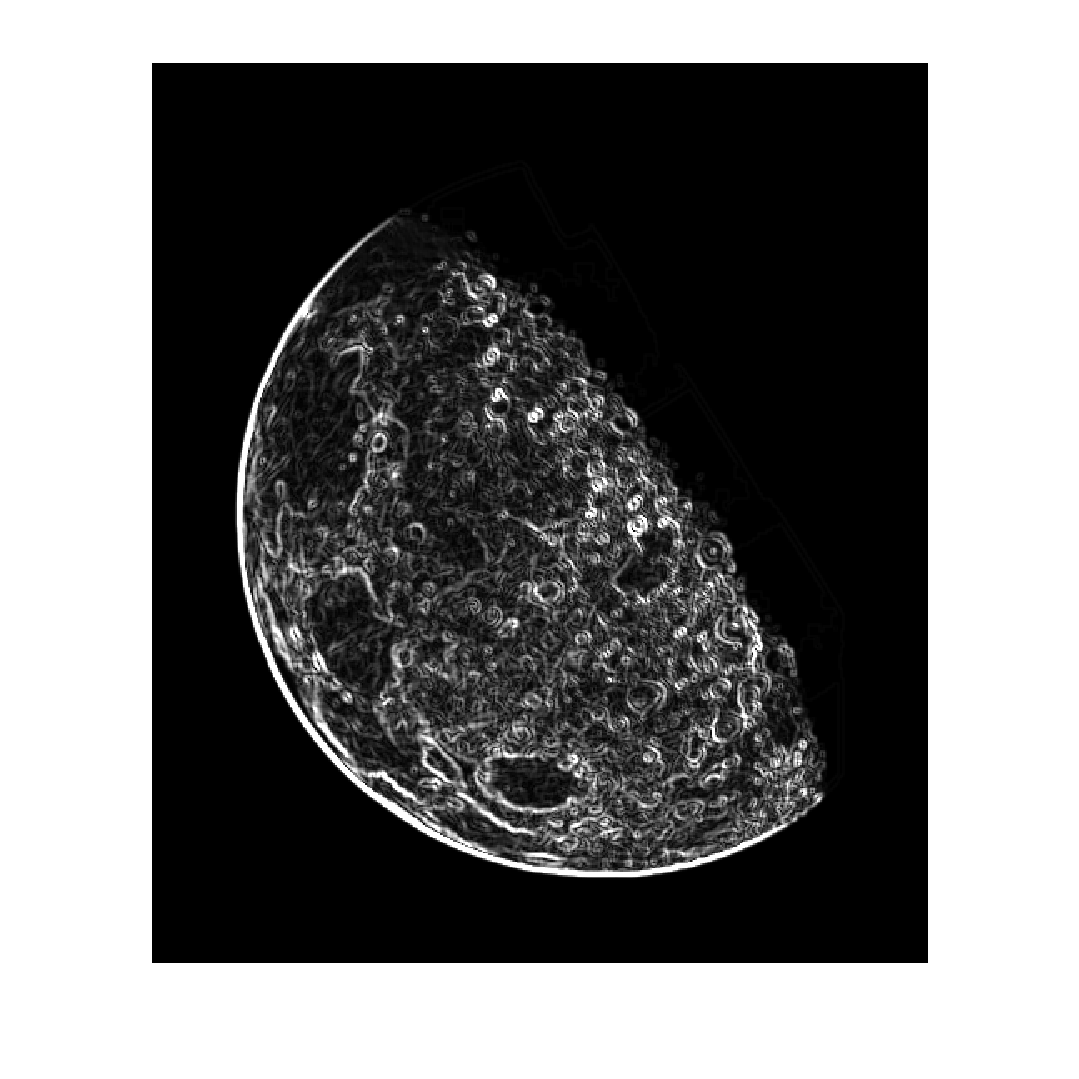
\includegraphics[width=\textwidth]{moonSharpened.eps}
  \caption{The Sobel operators applied to the previous figures, thus computing the gradient magnitude. Edges are now much more prominent as the gradient is the highest here.}
  \label{fig:moonSharp}
 \end{subfigure}
 \caption{Comparison of the original moon image and the moon image sharpened using \texttt{IPgradient}. It is clear that edges of objects (i.e. where the gradient magnitude is high) are much brighter and clearer than other objects.}
 \label{fig:moon}
\end{figure}
The MATLAB code to determine these images is the following:
\matlabexternal{IPgradient.m}

\subsection*{c - Order of operations}
We reasoned that generally there is a difference in the result when the order of the operations is concerned. We believe that this is due to the following reason. If a person would apply a sharpening filter first and subsequently a blur filter, pixels with a high gradient magnitude would first be highlighted and then slightly smoothed. However, if an blur filter is applied and then a sharpening filter, the overall gradient magnitude is lowered and therefore results in less highlights and deformations than would occur as in the former scenario. \newline
Therefore we figure that there will be a difference in the output images depending of the order of the blur and sharpen operations. We'd also reckon that generally images are more aesthetically pleasing when an image is first blurred and then sharpened. \newline 
We have tried to test this hypothesis by doing both operations and then comparing the results as figures~\ref{fig:angios} and figures~\ref{fig:blobs} illustrate. We can now conclude that there indeed is a difference between the images when the order of operations is changes. 
\begin{figure}[!Htb]
 \centering
 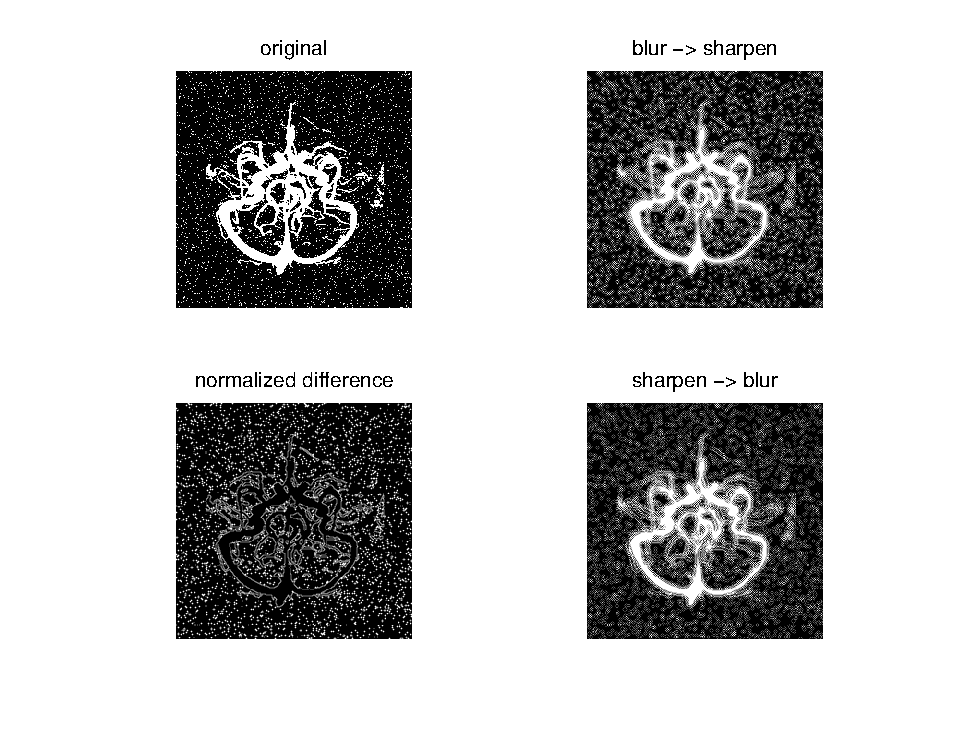
\includegraphics{angios.eps}
 \caption{An image of an angiogram with different orders in sharpening and blurring. A difference in resulting images can be observed. }
 \label{fig:angios}
\end{figure}
\begin{figure}[!Htb]
 \centering
 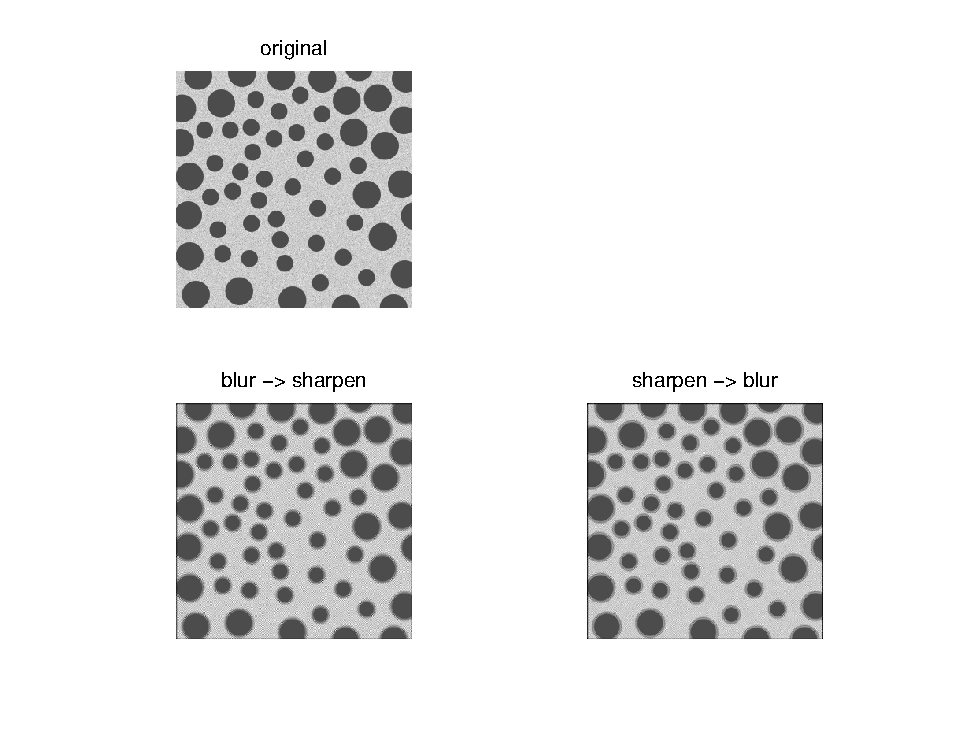
\includegraphics{blobs.eps}
 \caption{An image of blobs with different orders in sharpening and blurring. A difference in resulting images can be observed.}
 \label{fig:blobs}
\end{figure}
\clearpage
